\newpage

\subsubsection{UCS 6 - Selezione del monitoraggio di un'organizzazione o di un luogo specifico}

\begin{figure}[h]
\centering
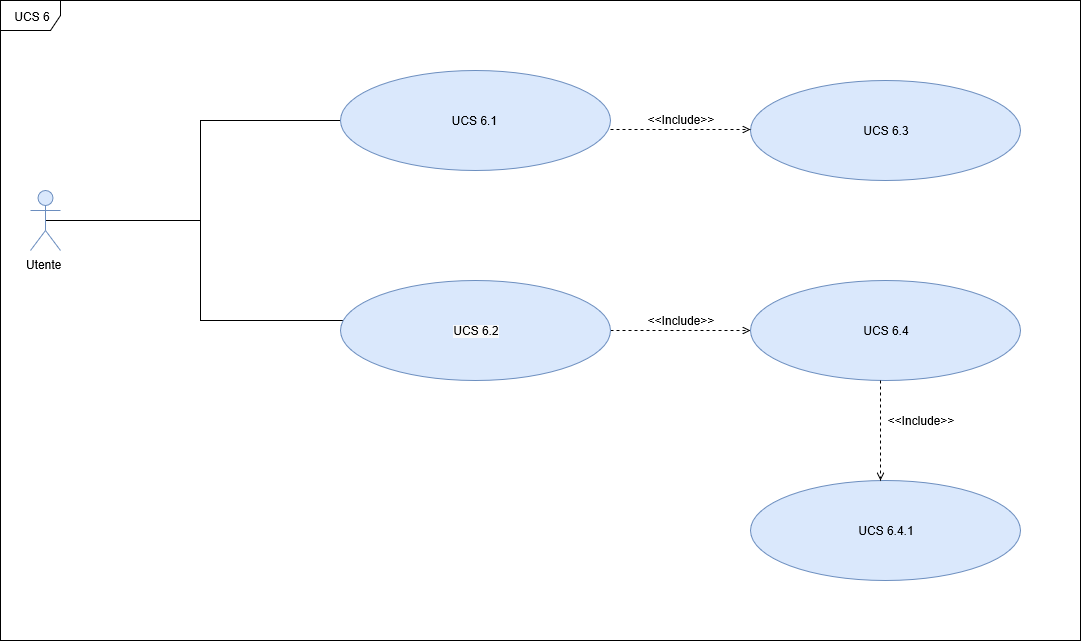
\includegraphics[scale=0.3]{sezioni/UseCase/Immagini/UCS6.png}
\caption{UCS 6 - Selezione del monitoraggio di un'organizzazione o di un luogo specifico}
\end{figure}

\begin{itemize}
	\item \textbf{Attori primari:} Amministratore visualizzatore
	\item \textbf{Precondizione:} L'amministratore deve essere autenticato\ap{G} presso il sistema e deve aver selezionato un'organizzazione.
	\item \textbf{Postcondizione:} L'amministratore avrà visualizzato il numero di utenti anonimi presenti in un'organizzazione o in un luogo specifico.
	\item \textbf{Scenario principale:} L'amministratore, dopo aver selezionato l'organizzazione, accede alla funzionalità di monitoraggio di un'organizzazione o di un luogo specifico. Poi potrà scegliere se visualizzare il numero di utenti anonimi presenti all'interno dell'organizzazione tramite la funzionalità di conferma o se scegliere la funzionalità di monitoraggio di un luogo specifico.
	\item \textbf{Flusso di eventi:}
\begin{enumerate}
	\item L'amministratore ha selezionato l'organizzazione [UCS 3];
	\item L'amministrazione deve selezionare la funzionalità di monitoraggio del luogo;
	\item L'amministratore può selezionare la funzionalità di conferma [UCS 6.1] o può selezionare la funzionalità di un luogo specifico [UCS 6.2].
\end{enumerate}
\item \textbf{Inclusioni:}
\begin{enumerate}
    \item UCS 3 - Selezione dell'organizzazione;
    \item UCS 6.1 - Selezione della funzionalità di conferma;
    \item UCS 6.2 - Selezione della funzionalità di monitoraggio di un luogo specifico.
\end{enumerate}
%\item \textbf{Estensioni:}  Visualizzazione di un messaggio che informa l'indisponibilità del server [?????];
\end{itemize}

\subsubsection{UCS 6.1 - Selezione della funzionalità di conferma}
\begin{itemize}
	\item \textbf{Attori primari:} Amministratore visualizzatore
	\item \textbf{Precondizione:} L'amministratore deve aver selezionato la funzionalità di monitoraggio del numero di utenti anonimi presenti in un'organizzazione o di un luogo specifico [UCS 6] oppure deve aver selezionato il luogo specifico che vuole monitorare [UCS 6.4].
	\item \textbf{Postcondizione:} All'amministratore verrà visualizzato il numero di utenti anonimi contenuti nell'organizzazione scelta [UCS 6.1.1] o di un luogo specifico [UCS 6.1.2].
	\item \textbf{Scenario principale:} L'amministratore, dopo aver selezionato la funzionalità di conferma, potrà visualizzare il numero di utenti anonimi presenti nell'organizzazione scelta o in un luogo specifico scelto.
	\item \textbf{Flusso di eventi:} 
	\begin{enumerate}
		\item L'amministratore ha scelto la funzionalità di conferma;
		\item L'amministratore visualizzerà gli utenti anonimi di un'organizzazione [UCS 6.1.1] o visualizzerà gli utenti anonimi di un luogo specifico [UCS 6.1.2].
	\end{enumerate}
%	\item \textbf{Inclusioni:}
%	\begin{enumerate}
 %   \item UCS 6.1.1 - Visualizzazione del numero di utenti anonimi di un'organizzazione;
  %  \item UCS 6.1.2 - Visualizzazione del numero di utenti anonimi di un luogo specifico.
	%\end{enumerate}
\end{itemize}

\subsubsection{UCS 6.2 - Selezione della funzionalità di monitoraggio di un luogo specifico}
\begin{itemize}
	\item \textbf{Attori primari:} Amministratore visualizzatore
	\item \textbf{Precondizione:} L'amministratore deve aver selezionato la funzionalità di monitoraggio del numero di utenti anonimi presenti in un'organizzazione o in un luogo specifico [UCS 6].
	\item \textbf{Postcondizione:} L'amministratore potrà visualizzare una lista con tutti i luoghi specifici presenti in un'organizzazione [UCS 6.3].
	\item \textbf{Scenario principale:} L'amministratore avrà scelto la funzionalità di monitoraggio di un luogo specifico che gli permetterà di visualizzare una lista di tutti i luoghi specifici dell'organizzazione scelta;
	\item \textbf{Flusso di eventi:} 
	\begin{enumerate}
		\item L'amministratore ha scelto la funzionalità di monitoraggio di un luogo specifico;
		\item L'amministratore visualizzerà una lista di tutti i luoghi specifici dell'organizzazione scelta [UCS 6.3].
	\end{enumerate}
	\item \textbf{Inclusioni:}
	\begin{enumerate}
		\item UCS 6.3 - Visualizzazione lista di tutti i luoghi specifici di un'organizzazione.
	\end{enumerate}
\end{itemize}


\subsubsection{UCS 6.3 - Visualizzazione lista di tutti i luoghi specifici di un'organizzazione}
\begin{itemize}
	\item \textbf{Attori primari:} Amministratore visualizzatore
	\item \textbf{Precondizione:} L'amministratore deve aver selezionato la funzionalità di monitoraggio di un luogo specifico [UCS 6.2].
	\item \textbf{Postcondizione:} L'amministratore avrà visualizzato una lista con all'interno tutti i luoghi specifici dell'organizzazione scelta.
	\item \textbf{Scenario principale:} All'amministratore verrà visualizzato una lista contenente tutti i luoghi dell'organizzazione scelta.
	\item \textbf{Flusso di eventi:} 
	\begin{enumerate}
		\item L'amministratore ha visualizzato una lista contenente il luogo specifico che vuole monitorare;
		\item L'amministratore sceglierà il luogo specifico [UCS 6.4].
	\end{enumerate}
	\item \textbf{Inclusioni:}
	\begin{enumerate}
		\item UCS 6.4 - Selezione di un luogo specifico.
	\end{enumerate}
\end{itemize}


\subsubsection{UCS 6.4 - Selezione di un luogo specifico}
\begin{itemize}
	\item \textbf{Attori primari:} Amministratore visualizzatore;
	\item \textbf{Precondizione:} L'amministratore deve aver visualizzato una lista di tutti i luoghi specifici dell'organizzazione scelta [UCS 6.3];
	\item \textbf{Postcondizione:} L'amministratore avrà scelto il luogo specifico in cui vuole fare il monitoraggio e potrà selezionare la funzionalità di conferma [UCS 6.1]
	\item \textbf{Scenario principale:} L'amministratore, da una lista contenente i luoghi dell'organizzazione, sceglierà il luogo specifico che vuole monitorare;
	\item \textbf{Flusso di eventi:} 
	\begin{enumerate}
		\item L'amministratore ha visualizzato una lista di tutti i luoghi specifici [UCS 6.3];
		\item L'amministratore sceglie il luogo specifico che vuole monitorare;
		\item L'amministratore potrà selezionare la funzionalità di conferma [UCS 6.1] per poter visualizzare il numero di utenti anonimi di un luogo specifico [UCS 6.1.2].
	\end{enumerate}
	\item \textbf{Inclusioni:}
	\begin{enumerate}
		\item UCS 6.3 - Visualizzazione lista di tutti i luoghi specifici di un'organizzazione;
		\item UCS 6.1 - Selezione della funzionalità di conferma;
	%	\item UCS 6.1.2 - Visualizzazione del numero di utenti anonimi di un luogo specifico.
	\end{enumerate}
\end{itemize}

\subsubsection{Panoramica UCS 6.1.1/6.1.2}

\begin{figure}[h]
	\centering
	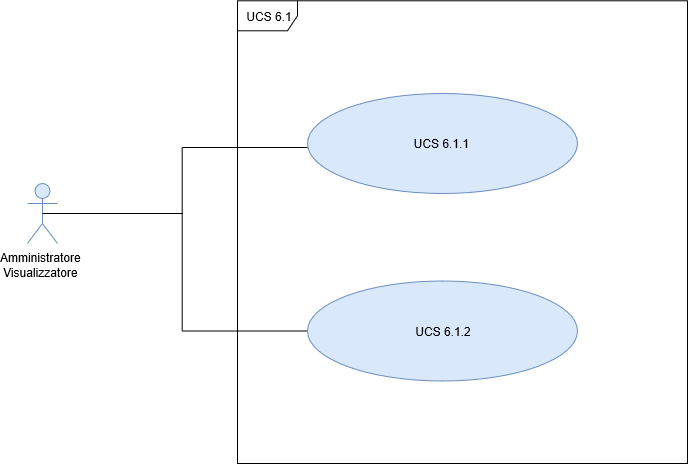
\includegraphics[scale=0.3]{sezioni/UseCase/Immagini/UCS6_1.png}
	\caption{Visualizzazione del numero di utenti anonimi di un'organizzazione o di un luogo specifico}
\end{figure}


\subsubsection{UCS 6.1.1 - Visualizzazione del numero di utenti anonimi di un'organizzazione}
\begin{itemize}
	\item \textbf{Attori primari:} Amministratore visualizzatore
	\item \textbf{Precondizione:} L'amministratore, dopo aver selezionato la funzionalità di monitoraggio del numero di utenti anonimi presenti in un'organizzazione o di un luogo specifico [UCS 6], deve aver selezionato la funzionalità di conferma [UCS 6.1].
	\item \textbf{Postcondizione:} L'amministratore avrà visualizzato il numero di utenti anonimi contenute nell'organizzazione scelta.
\end{itemize}

\subsubsection{UCS 6.1.2 - Visualizzazione del numero di utenti anonimi di un luogo specifico}
\begin{itemize}
	\item \textbf{Attori primari:} Amministratore visualizzatore
	\item \textbf{Precondizione:} L'amministratore, dopo aver scelto il luogo specifico [UCS 6.4], deve aver selezionato la funzionalità di conferma [UCS 6.1].
	\item \textbf{Postcondizione:} L'amministratore avrà visualizzato il numero di utenti anonimi contenuto nel luogo specifico presente nell'organizzazione scelta.
\end{itemize}



